\section{Project preliminaries} \label{sec:2}
\subsection{Task description} \label{subsec:2.1}
The goal of the project work was to explore the $p_{T}$ transverse momentum dependence of the $v_{2}$ elliptic flow coefficient using real, but simplified observational data, presented us in ROOT \texttt{Tree} format\footnote{\url{https://root.cern/manual/trees/}}$^{,}$\footnote{\url{https://root.cern.ch/doc/master/classTTree.html}}. The calculation of $v_{2}$ was needed to be done for a single, global centrality class in the interval of $0\%$ to $92\%$ as a function of the $p_{T}$ transverse momentum, where

\begin{figure}[t]
	\centering
	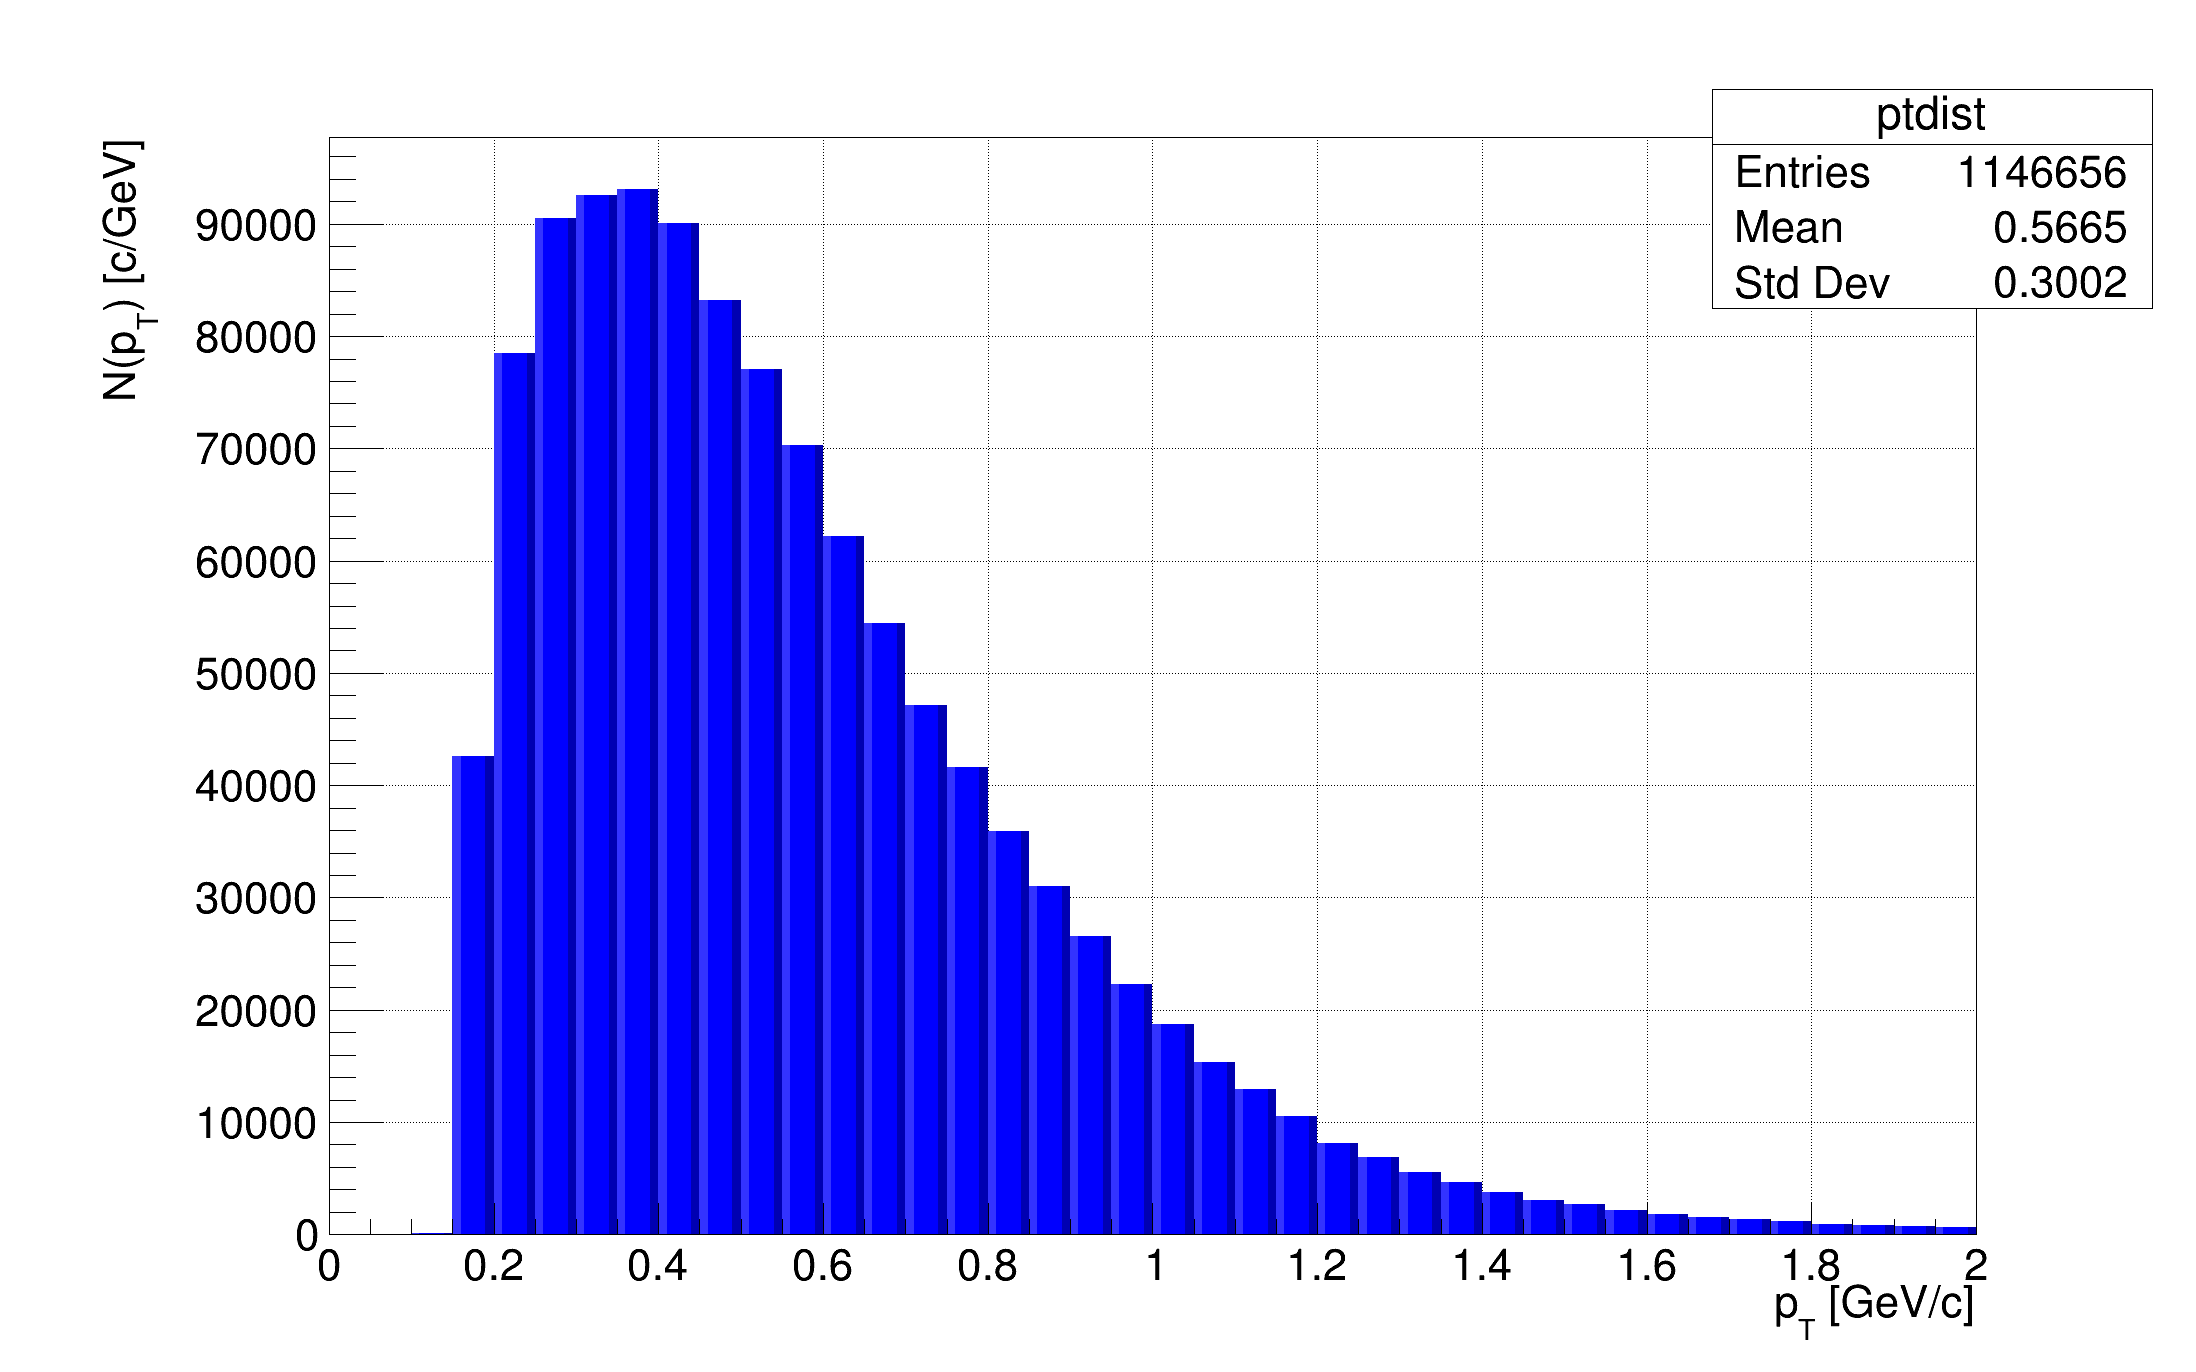
\includegraphics[width=\textwidth]{ptdist.png}
	\captionof{figure}{The $p_{T}$ transverse momentum distribution in the experimental data. The reason for the interest in the transverse momentum can be simply understood. The momentum of the colliding particles are entirely parallel to the reaction plane, when they circulating inside the pipe of a collider. After the collision, spectator particles will travel down the pipe, while particles in the collision zone will scatter into every direction. This means that only particles in this interesting region will have a momentum component perpendicular to the reaction plane, thus studying focusing on particles with non-zero $p_{T}$ values will ensure that only particles from the collision zone will be taken into account in our analysis.}\label{fig:1}
\end{figure}

\begin{equation*}
	0\ \mathrm{GeV}/\mathrm{c} < p_{T} < 2\ \mathrm{GeV}/\mathrm{c}.
\end{equation*}
The width of the $p_{T}$ bins were supposed to be $50\ \mathrm{MeV}/\mathrm{c}$, which implies the existence of $40$ bins for the total of $2\ \mathrm{GeV}/\mathrm{c}$ wide observational range.

The observed $v_{2}^{\mathrm{obs}}$ values needed to be corrected for the event plane resolution $R$ to obtain the real $v_{2}^{\mathrm{real}}$ values of the measurements.

At last I've compared the results to real values (which could be seen eg. on the upper panel of Fig. (2) in \citep{Collaboration2003}). It should be also noted that in our dataset only pions were present, thus all results should be treated accordingly when they're compared to values in the literature.

\subsection{Solution strategy} \label{subsec:2.2}
The main goal of the project was to determine the $v_{2} \left( p_{T} \right)$ function that describes the connection between the transverse momentum and the elliptic flow parameter. The $v_{2}$ value is proportional to the angle distribution, which relation can be expressed using the \eqref{eq:1.1} definition as

\begin{equation} \label{eq:2.1}
	\Df{N}{\phi}
	\,\propto\,
	1 + 2 v_{2} \cos \left( 2 \phi \right).
\end{equation}
The $\phi$ angle can be calculated according to \eqref{eq:1.2}, where the $\Psi$ reaction plane angle is given in the provided dataset. The $\phi_{0}$ raw angle can be simply obtained from the momentum values eg. as

\begin{equation} \label{eq:2.2}
	\phi_{0}
	=
	\operatorname{atan2} \left( p_{y}, p_{x} \right)
\end{equation}
At the end the $\phi$ values should be normalized into the interval of $\left[ -\frac{\pi}{2}, \frac{\pi}{2} \right]$ eg. using the following simple algorithm:

\begin{equation}
	\phi
	=
	\begin{cases}
		\phi + 2 \pi & \text{if } \phi < -\pi \\
		\phi - 2 \pi & \text{if } \phi > \pi \\
		\phi + \pi & \text{if } \phi < -\pi/2 \\
		\phi - \pi & \text{if } \phi > \pi/2.
	\end{cases}
\end{equation}
Given the proportion above in \eqref{eq:2.1}, one can find the value of $v_{2}^{\mathrm{obs}}$ by fitting a

\begin{equation} \label{eq:2.3}
	f
	=	
	a + 2 * b \cos \left( 2 \phi \right)
\end{equation}
parametrized trigonometric function on the angle distribution of particles. To explore the $p_{T}$ dependence of the $v_{2}$ coefficient, one has to bin the $p_{T}$ space, determine the angle distribution for all $p_{T}$ bins and obtain the $v_{2}$ value for each of them by fitting the function defined in \eqref{eq:2.3}. The value of the $v_{2}^{\mathrm{obs}}$ parameter will be then calculated as

\begin{equation}
	v_{2}^{\mathrm{obs}}
	=
	\frac{b}{a}.
\end{equation}
The bin width chosen for this project was $50\ \mathrm{MeV}/\mathrm{c}$. At the end this value has to be scaled by the event plane resolution to get the final value of $v_{2}$ as

\begin{equation}
	v_{2}
	=
	\frac{v_{2}^{\mathrm{obs}}}{R}.
\end{equation}
Event plane resolution is defined as a function of centrality and was given in a supplementary dataset. Since I was intended to work in a single centrality group, a smart average value of the event plane resolution should have been found. I've simply calculated the average of the resolution values, weighted by the widths of the centrality bins to obtain an approximate value of

\begin{equation*}
	R
	\approx
	0.3265
\end{equation*}
for the average.

\begin{figure}[t!]
	\centering
	\includegraphics[width=\textwidth]{{ntrackdist.png}}
	\captionof{figure}{The histogram shows the number of events for different track numbers in the data. The average number of tracks per event are $11-12$ approximately.}\label{fig:2}
\end{figure}

\subsection{Project code} \label{subsec:2.3}
\subsubsection{Initial base}
A code base was provided for the project that contained some essentials to help us successfully complete the assignment. This package contained the framework that defines the structure of the data tree class, as well as lends a helping hand to easily process files encoded in this format.

The given code also contains a basic analysis routine that iterates over all events and particle tracks and thus allows us to collect all relevant entries from the dataset. Any further project codes were advised to be built on top of this foundation.

The provided data tree is organized into the following structure:

\begin{align*}
	\mathrm{Tree}
	=
	\big\{& \\
	&\quad \text{event}_{1} :
		\left\{ \text{track}_{1}^{1}, \text{track}_{2}^{1}, \dots, \text{track}_{N_{1}}^{1} \right\},\\
	&\quad \text{event}_{2} :
		\left\{ \text{track}_{1}^{2}, \text{track}_{2}^{2}, \dots, \text{track}_{N_{2}}^{2} \right\},\\
	&\quad \vdots \\
	&\quad \text{event}_{n} :
		\left\{ \text{track}_{1}^{n}, \text{track}_{2}^{n}, \dots, \text{track}_{N_{n}}^{n} \right\}\\
	\big\}&.
\end{align*}
The provided dataset in our case contains $100\,000$ events, with a variable number of tracks in each of them. The average number of tracks for an event is $11-12$. Event-level properties data contain the centrality, $z$-vertex location, $\Psi$ reaction plane angle and track number values, while track-level properties contain the particle momenta, energy, charge and some other -- here not relevant -- quantities.

\subsubsection{Final code}
The infamous ROOT library, used extensively by nuclear- and particle physics researchers all around the world for decades was utilized here to implement the final project code. However this software is considered to be heavily bloated, it contains all useful numerical methods and techniques that were needed to finish the task. Nonetheless to mention, that the data files were also stored in a ROOT format file that trivially ROOT can handle the most conveniently.

I've refractored almost the entirety of the analysis code, turning it into a functional code, instead of having a single \texttt{main()} method. This made the final code much more modular and clear to work with.

For the fitting of the angle distribution I've used the built-in method of ROOT for $1$D histogram fitting, the \texttt{TH1::Fit()} function. This produced high precision results for lower $p_{T}$ bins, but also high errors in the higher $p_{T}$ regime. The results of some fits can be seen on (\ref{fig:3}). The upper two panel shows fits for angle distributions on low $p_{T}$ values, while the bottom panels shows fits in the high $p_{T}$ regime.

\begin{figure}[t!]
	\centering
    \begin{subfigure}[b]{0.475\textwidth}
		\centering
		\includegraphics[width=\textwidth]{{fit_4.png}}
		\caption[]%
		{$4$th $p_{T}$ bin}
		\label{fig:3.1}
	\end{subfigure}
	\hfill
	\begin{subfigure}[b]{0.475\textwidth}  
		\centering 
		\includegraphics[width=\textwidth]{{fit_7.png}}
		\caption[]%
		{$7$th $p_{T}$ bin}   
		\label{fig:3.2}
	\end{subfigure}
	\vskip\baselineskip
	\begin{subfigure}[b]{0.475\textwidth}   
		\centering 
		\includegraphics[width=\textwidth]{{fit_36.png}}
		\caption[]%
		{$36$th $p_{T}$ bin}    
		\label{fig:3.3}
	\end{subfigure}
	\hfill
	\begin{subfigure}[b]{0.475\textwidth}   
		\centering 
		\includegraphics[width=\textwidth]{{fit_38.png}}
		\caption[]%
		{$38$th $p_{T}$ bin}  
		\label{fig:3.4}
	\end{subfigure}
	\caption[]%
	{The fitted angle distributions for different $p_{T}$ bins. The larger errors in the higher $p_{T}$ regime can be attributed to the relatively small number of data in that interval. The difference in the number of data points between the high and low $p_{T}$ regime is a $\approx 10^{2}$ multiplier.} 
	\label{fig:3}
\end{figure}